\chapter{Objetivos}\label{cap.objetivos}
En este punto ya hemos introducido el contexto en el que desarrolla el trabajo, es momento de describir los objetivos que se han tratado de alcanzar, los requisitos para las soluciones desarrolladas y la metodología seguida para su consecución.

\section{Objetivos}
La meta de este proyecto consiste en la creación de dos nuevas prácticas de sistemas robóticos para el entorno docente JdeRobot-Academy, una primera que consistirá en seguimiento de caras a través de una cámara y otra sobre auto localización de un robot basada en láser. Para cada una de ellas se creará la infraestructura necesaria y una solución de referencia.

En primer lugar, la práctica de seguimiento de caras utilicará una cámara móvil montada en un cuello mecánico, la cual puede apuntarse hacia varias direcciones, para que el alumno ponga en práctica sus conocimientos de segmentación de imagen buscando posibles caras de personas en la imágenes que le sirve dicha cámara, y generando órdenes para los motores de la cámara de modo que esta siga con la mirada el movimiento de la persona que tiene delante.

La segunda práctica creada es sobre un robot móvil y busca resolver un problema de auto localización basada en láser, de manera que dicho robot sepa en todo momento su posición y orientación en el entorno que le rodea, valiéndose únicamente de un sensor láser incorporado.

\section{Requisitos} 
El software desarrollado, además de proporcionar las dos prácticas deseadas, deberá cumplir estos requisitos de partida del proyecto:

\begin{enumerate}
	\item El sistema operativo que se empleará para este proyecto será Ubuntu 16.04 LTS.
	\item Se hará uso del middleware robótico JdeRobot en su versión 5.6.1. El uso de esta plataforma simplifica el desarrollo del comportamiento del robot.
	\item Se hará uso de OpenCV3 en la práctica de seguimiento de caras.
	\item En el ejercicio de localización basada en láser se usará \textit{ROS-Kinetic} y todas las simulaciones se realizarán en el simulador Gazebo, en concreto en la versión 7.9.0. 
	\item El lenguaje de desarrollo empleado para crear los distintos componentes será Python, en concreto en su versión 2.7.12. Por compatibilidad con JdeRobot-5.6.1 y de éste con el middleware ROS \textit{Kinetic} no se ha usado Python-3.x
	\item Las soluciones han de ejecutar algoritmos que funcionen en tiempo real, de manera que deberán ser eficientes y ejecutar movimientos suaves.
\end{enumerate}

\section{Metodología}
La elaboración de este trabajo podría descomponerse en un conjunto de iteraciones con varias fases, en cada una de las cuales se establecía una reunión con el tutor para determinar los subobjetivos siguientes, planificar cómo abordarlos, analizar los posibles problemas y corregir fallos. Así, se ha conseguido un desarrollo fluido y completo, asentando los conocimientos y despejando las dudas que surgían a lo largo de los meses que se dedicó al trabajo.

Parte del seguimiento lo hemos hecho utilizando herramientas de apoyo, como la bitácora semanal en la Wiki de JdeRobot \footnote{\url{https://jderobot.org/Cawadallah-tfg}} donde periódicamente se redactaban los avances realizados y se añadían vídeos demostrativos de lo conseguido, imágenes representativas y texto descriptivo. El código asociado a los avances se almacenó en un repositorio personal de GitHub\footnote{\url{https://github.com/cawadall/Academy}}\footnote{\url{https://github.com/cawadall/JdeRobot}}, al que el tutor ha podido acceder en todo momento para aportar realimentación y favorecer el progreso.

Se ha optado por seguir el modelo de desarrollo en espiral creado por Barry Boehm, el cual hemos creído que se adaptaba perfectamente a nuestras necesidades, permitiéndonos separar el comportamiento final en varias sub-tareas más sencillas, a la par que disponer de flexibilidad ante cambios en los requisitos, algo bastante común a medida que avanzaba el desarrollo. Con él, conseguimos una resolución temprana de riesgos y poder definir la arquitectura en las fases iniciales, todo ello basado en un proceso continuo de verificación de la calidad.

\begin{figure}[H]
  \begin{center}
    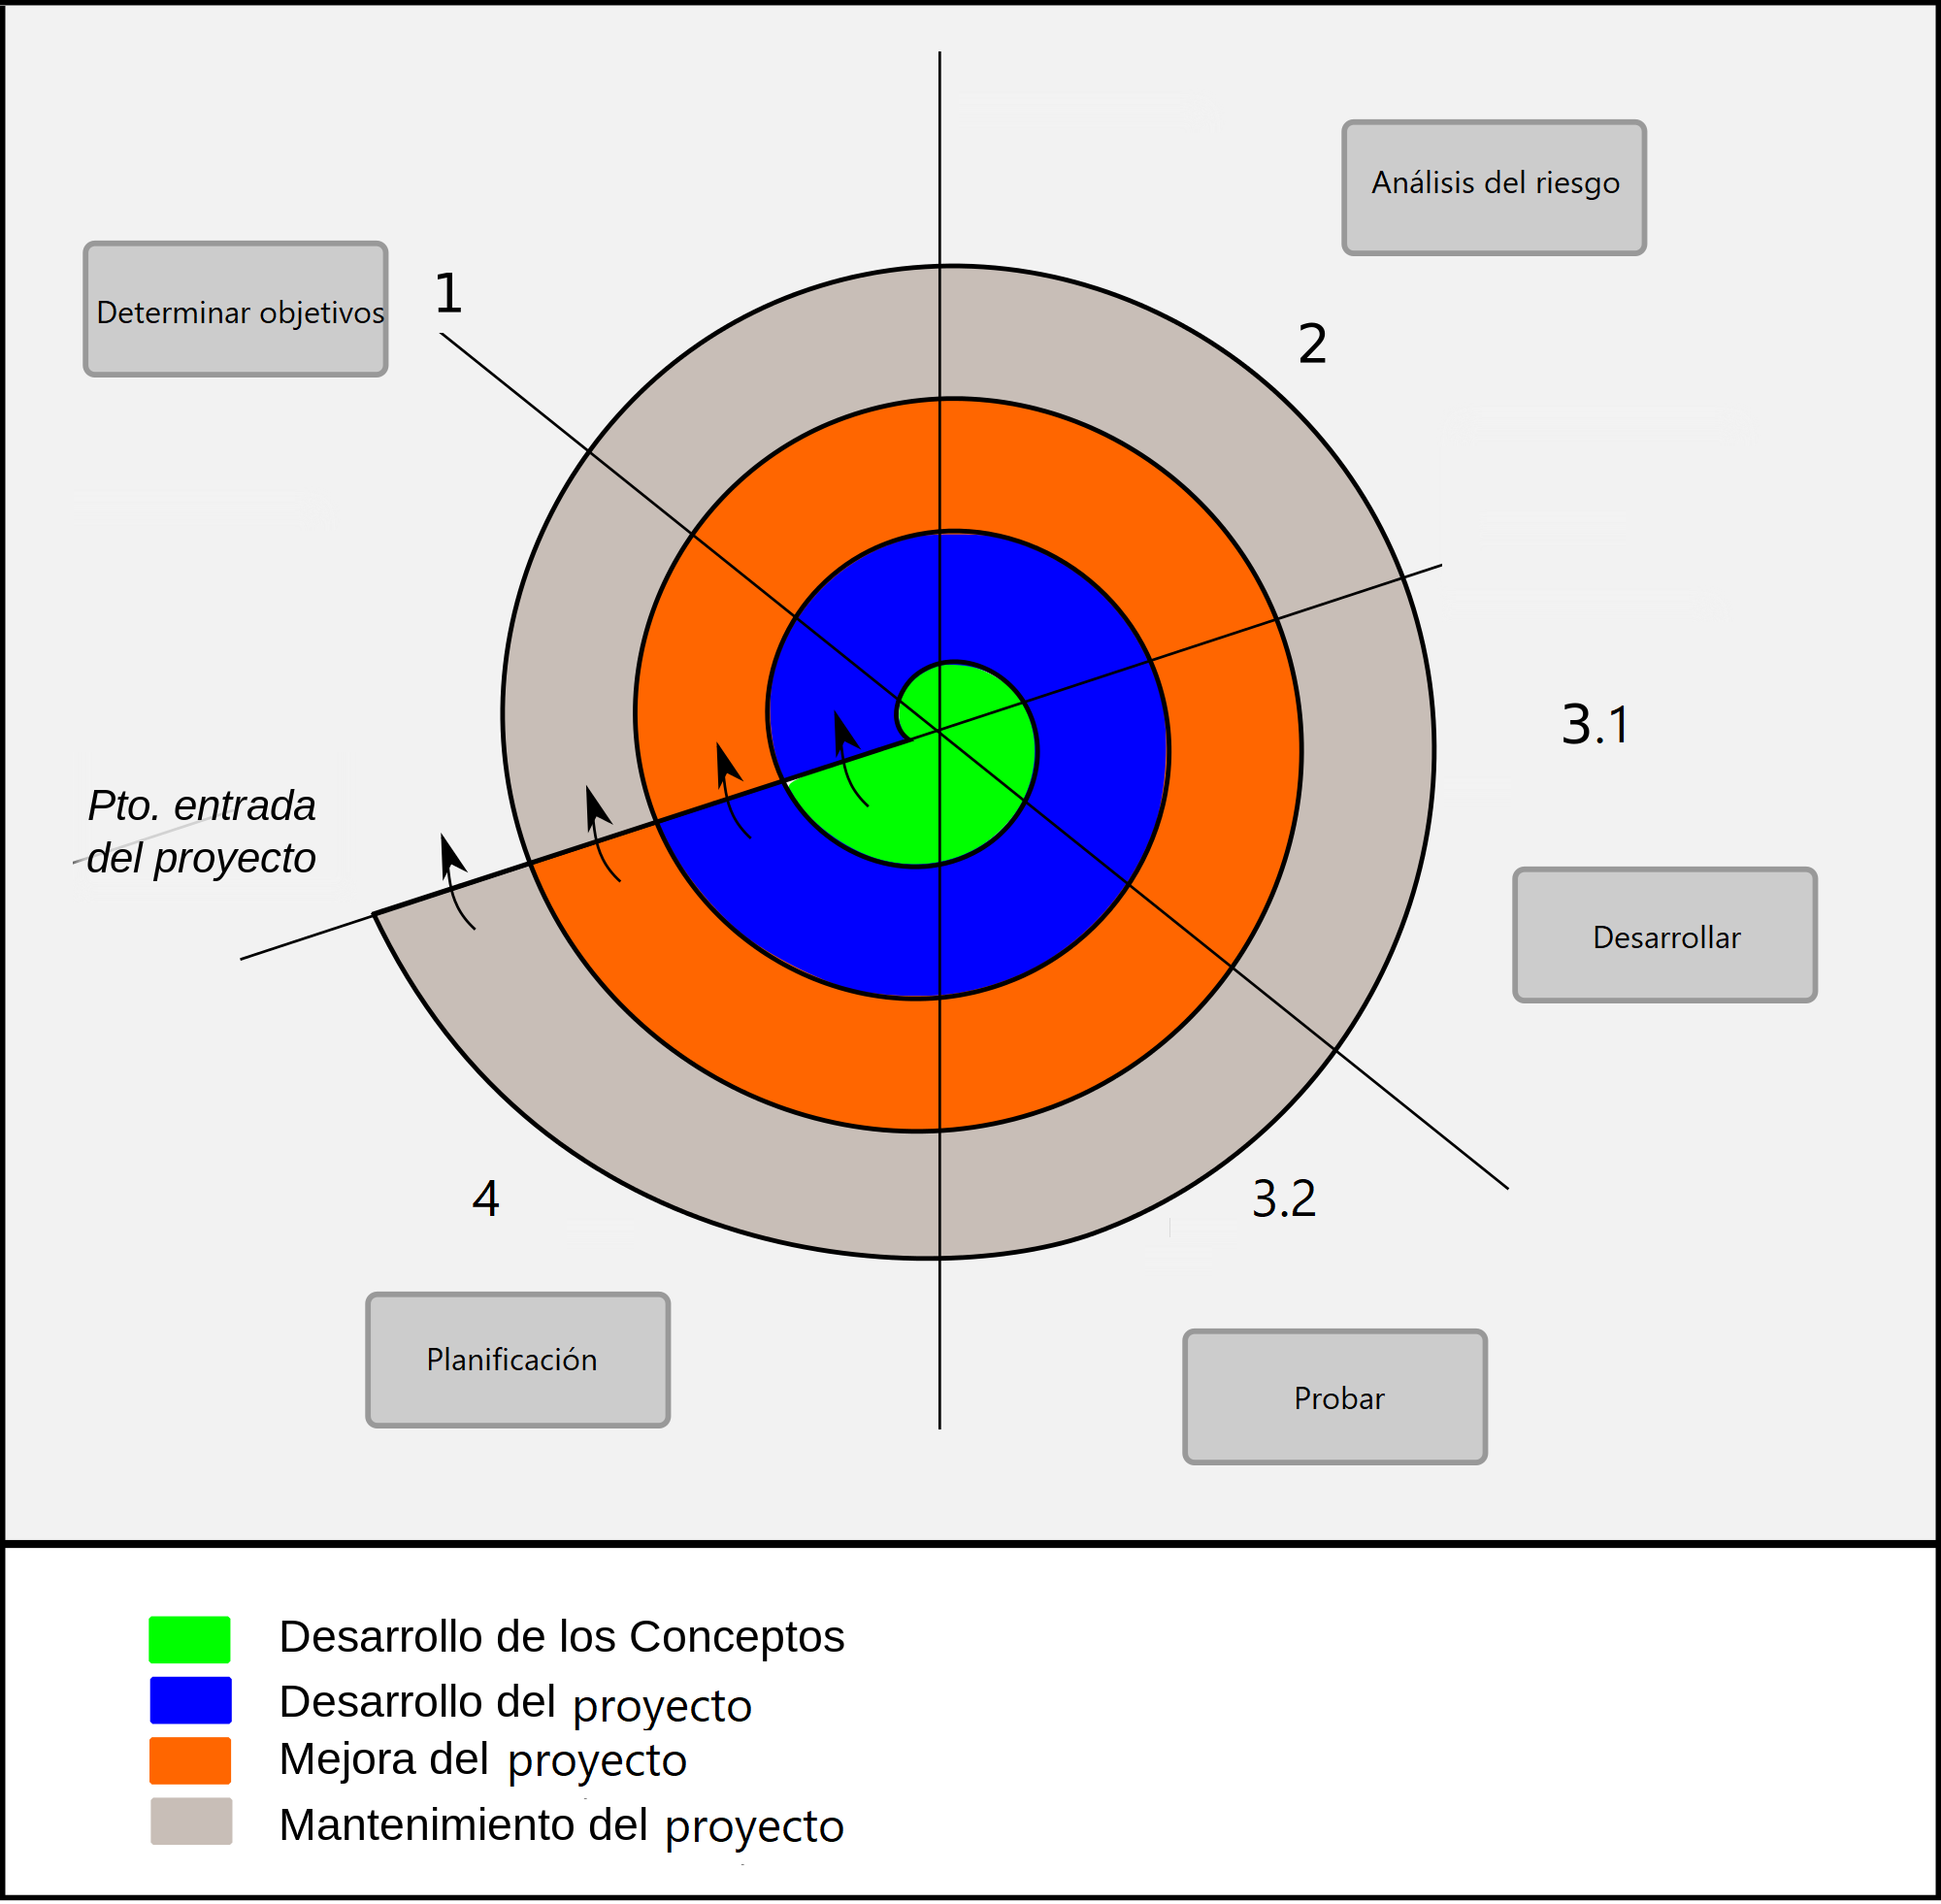
\includegraphics[width=0.9\linewidth]{figures/modelo_espiral.png}
		\caption{Modelo de desarrollo en espiral}
		\label{fig.espiral}
		\end{center}
\end{figure}

Como se puede ver en la \textbf{Figura 2.1}, este modelo de ciclo de vida permite ir obteniendo prototipos funcionales en primera instancia, luego mejorar el prototipo conseguido y, por último, pulir los detalles para cubrir todos los requisitos.  Así, se realiza el trabajo de forma incremental, en forma de ciclos con cuatro fases bien definidas:

\begin{itemize}
	\item[--] \textbf{Determinar objetivos}: en esta primera fase del ciclo se definen las metas que se deben conseguir para que una vez completadas se pueda dar por finalizado el mismo.
	\item[--] \textbf{Análisis del riesgo}: en la segunda fase se evalúa qué problemas es posible encontrarse al empezar el desarrollo, y se piensa en cómo abordarlos.
	\item[--] \textbf{Desarrollar y probar}: en la tercera fase es en la que, tras evaluar los riesgos, se procede al propio desarrollo del trabajo, además de las correspondientes pruebas para verificar su correcta funcionalidad.
	\item[--] \textbf{Planificación}: en esta última fase se valoran los resultados obtenidos en el ciclo y se planifican las siguientes etapas del proyecto.
\end{itemize}

\section{Plan de trabajo}
Para lograr los objetivos descritos, se han seguido las siguientes etapas de trabajo:

\begin{itemize}
	\item[--] \textbf{Familiarización con el entorno JdeRobot}. Tras la descarga e instalación del software  involucrado, incluyendo dependencias, simulador y bibliotecas necesarias, se tratará de entrar en contacto con el entorno JdeRobot modificando y pulimentando algunas prácticas existentes para añadir mejoras, por ejemplo, en sus interfaces gráficas.
	\item[--] \textbf{Toma de contacto con el simulador Gazebo}. En esta etapa se han estudiado distintos ejemplos disponibles en la web de Gazebo\footnote{\url{http://gazebosim.org/tutorials}} y de JdeRobot. Además, se ha estudiado el funcionamiento básico de los \textit{plugins}  que Gazebo emplea para controlar los robots, sus sensores y sus actuadores. Esto ha implicado la investigación del lenguaje de programación C++, el cual también ayudará a comprender los \textit{plugins} ROS.
	\item[--] \textbf{Estudiar las bibliotecas involucradas}, entre las cuales destacan OpenCV, Threading, NumPy y PyQt5.
\end{itemize}

Una vez aquí, se centrarán los esfuerzos en…

\begin{itemize}
	\item[--] \textbf{Desarrollo de la infraestructura para la práctica de seguimiento de caras}. Manejo de los \textit{drivers} involucrados para el control de los motores y de la cámara. Se creará el nodo académico que albergará el código del estudiante. También se creará una versión de la práctica a través de Jupyter.
	\item[--] \textbf{Programación de una solución de referencia para el seguimiento de caras}.
	\item[--] \textbf{Preparación de la infraestructura para el ejercicio de autolocalización basada en láser}. Se desarrollará el \textit{driver} para el robot simulado. Se creará el nodo académico que alberga el código del estudiante, además de un cuadernillo de Jupyter con la misma funcionalidad.
que alberga alternativamente el código del estudiante.
	\item[--] \textbf{Programación de una solución de referencia para la autolocalización}.
	\item[--] \textbf{Obtención de conclusiones} acerca de lo estudiado, con las cuáles completar la formación en el campo.
\end{itemize}